% Created 2022-06-28 Tue 13:24
% Intended LaTeX compiler: pdflatex
\documentclass[a4paper, 11pt, twocolumn]{article}
\usepackage[utf8]{inputenc}
\usepackage[T1]{fontenc}
\usepackage{graphicx}
\usepackage{longtable}
\usepackage{wrapfig}
\usepackage{rotating}
\usepackage[normalem]{ulem}
\usepackage{amsmath}
\usepackage{amssymb}
\usepackage{capt-of}
\usepackage{hyperref}
                \usepackage{amsmath}
\usepackage{cleveref}

                \input{/home/casper/orgfiles/tex_templates/fun_article_template.tex}
                \addbibresource{/home/casper/library.bib}

\usepackage[english]{babel}
\author{Casper van Elteren, Rick Quax, Peter Sloot}
\date{\today}
\title{An information theory perspective on tipping points in dynamical networks}
\begin{document}

\maketitle
\lettrineabstract{Abrupt, system-wide transitions can be endogenously generated by seemingly stable networks of interacting dynamical units, such as mode switching in neuronal networks or public opinion changes in social systems. However, it remains poorly understood how such `noise-induced transitions' are generated by the interplay of network structure and dynamics on the network. Here we use information theory to discover how such "tipping points" can emerge in dynamic networks governed by the Boltzmann-Gibbs distribution. We identify two key roles for nodes in for tipping behavior to occur. In the initial phase, nodes with low degree pass on short-lived fluctuations to neighboring nodes, causing a domino-effect making neighboring nodes more dynamic. Conversely, towards the tipping point we identify other nodes whose state information becomes part of the long-term memory of the system. In addition, we show that identifying the different roles enables performing different types of targeted interventions that make tipping points more (less) likely to begin or to lead to systemic change. In general this progression depends on the combination of network structure and dynamics, which can be discovered using our methodology. This opens up possibilities for understanding and controlling endogenously generated metastable behavior.}

\section{Introduction}
\label{sec:orgd6a1d62}
Multistability  is  an   important  characteristic  in  many
real-world  complex systems  \cite{Ladyman2013,vanNes2016}. It
entails the phenomenon whereby  a system under the influence
of noise  explore its  state space on  different timescales.
For example, the  neural network's of the  brain can produce
various   oscillations   in    different   cognitive   modes
\cite{Fries2015}.  Similarly,  the life  cycle  of  a cell  is
tightly regulated between two bistable states of mitosis and
interphase \cite{Kandel2000}.  Other examples exist  on larger
scales such  as the  emergence of multistability  in opinion
dynamics \cite{Galam2020}, or the multistability of ecosystems
or climate systems \cite{1986,Wunderling2021}. Multistability
allows for  a system  to absorb  and adapt  to noise-induced
fluctuations,  yielding  its  universal  character  in  many
complex systems \cite{Ladyman2013}.

The mechanisms  underlying these  transitions are  often not
well understood. It is of vital importance to understand the
underlying  processes  that  cause  metastable  behavior  to
quantify the impact of noise on complex systems.

Here, we  consider dynamical systems consisting  of a static
network  where the  states of  the nodes  are governed  by a
Boltzmann-Gibbs distribution (\cref{fig:introduction}). This
type of  model has  been used  to describe  a wide  range of
behaviors  such   as  neural   dynamics  \cite{Hopfield1982b},
opinion dynamics, ferromagnetic spins [\cite{Glauber1963}, and
organized criminal gang interactions \cite{DOrsogna2015a}.

In  this class  of models,  each node  chooses its  state in
equilibrium with  the potential  induced by  its neighboring
states.  In  physical  applications this  potential  is  the
classic energy  potential, but in other  applications it can
be   interpreted,  for   instance   as  frustration   level,
homophily, or more broadly speaking,  a fitness score of the
node  state given  its neighbors.  The second  ingredient in
this model is a global  'temperature' which is essentially a
noise level: at zero noise  a node always picks the absolute
minimum energy  state, whereas the higher  this noise level,
the more likely it is that high energy states are chosen.

For low noise  levels, it is common for  systems governed by
the  Boltzmann-Gibbs  distribution   to  exhibit  metastable
behavior because of the existence of multiple (local) minima
in the system's potential (\cref{fig:introduction}{a-c}). In
finite systems  and non-zero temperature, there  is a finite
probability  that the  system  moves  (eventually) from  one
local  minimum to  another. Without  loss of  generality, in
this  paper we  illustrate our  method using  the well-known
kinetic  Ising spin  model  without  external forces.  Here,
nodes have  only two possible  states: +0 and +1.  At system
level, there are two global minima: all nodes in state +0 or
all nodes in  state +1 (\cref{fig:introduction}{c}). Between
these  two   system  states   lies  a   'potential  barrier'
(\cref{fig:introduction}{a-inset}):  many possible  paths of
system states which connect the two systemic minima, but all
of which have  a growing potential, making  these paths less
likely than paths of similar length that remain close to one
of  the  minima.  The  peak of  this  potential  along  each
crossing path lies, informally  speaking, at a 'checkerboard
pattern':  each node  being  maximally  different from  (the
majority of)  its neighbors.  We refer to  this peak  as the
'tipping point'.

The crucial  point here  is that  the network  structure can
make systemic  transitions much more likely  than without it
\cite{Harush2017a,Gao2016,Wunderling2020,Wunderling2021}.
Without  network  effects,  each  node  has  an  independent
probability of choosing the (unlikely) high potential state.
The probability  that all nodes  in the system happen  to do
this simultaneously (thereby  transitioning the system state
to another potential minimum)  decreases to zero rapidly (as
\(\mathcal{O}(e^{-N^2})\)  for dense  networks). This  means
that transitions  become unlikely  for all but  the smallest
systems.  With  network  effects, however,  transitions  can
potentially occur along  a path of nodes that  form a domino
effect. That  is, the  first node  choosing randomly  a high
potential state makes the  same state transition more likely
for all of  its neighbors. For some of  these neighbors this
new situation may  suffice to make the  same transition with
(almost)  equal likelihood  as the  first node,  and so  on,
until the tipping point has  been reached. The likelihood of
such  a  transition  is  much higher  than  without  network
effects (up  to \(\mathcal{O}(e^{-N})\)).  This is  still an
exponentially decaying function of system size, highlighting
the  fact that  such  noise-induced  transitions still  only
occur in finite-size systems, but exceedingly more likely.

Here, we present a method to uncover the network percolation
process    that   facilitates    endogenous,   noise-induced
transitions. The  computational method only  requires access
to  cross-sections of  time-series  of  observations of  the
system, meaning that it is broadly applicable.

The  method consists  of  analyzing two  key features  using
information flows  of a system:  the time of  the short-term
information  decay,  and  the long-term  information  level.
Here, the contribution  of each node to  the system dynamics
over  time  are  considered.   The  results  highlight  that
short-lived   correlations   measured  by   Shannon   mutual
information shared  between and  node and the  entire system
(\(I(s_i  : S^t)\))  are  essential to  absorb and  transfer
noise through the  system. After the majority  of the system
crosses  the  tipping  point,  a new  local  equilibrium  is
established. These long-term  correlations are essential for
the system  to maintain  its metastable state.  The approach
differs from  traditional approaches  that focus on  how the
system  as a  whole approaches  a tipping  point. Here,  the
mechanism  underlying  \emph{how}  local  connectivity  of  nodes
contribute  to the  system  dynamics can  be understood  and
analyzed.

\begin{figure*}
\centering
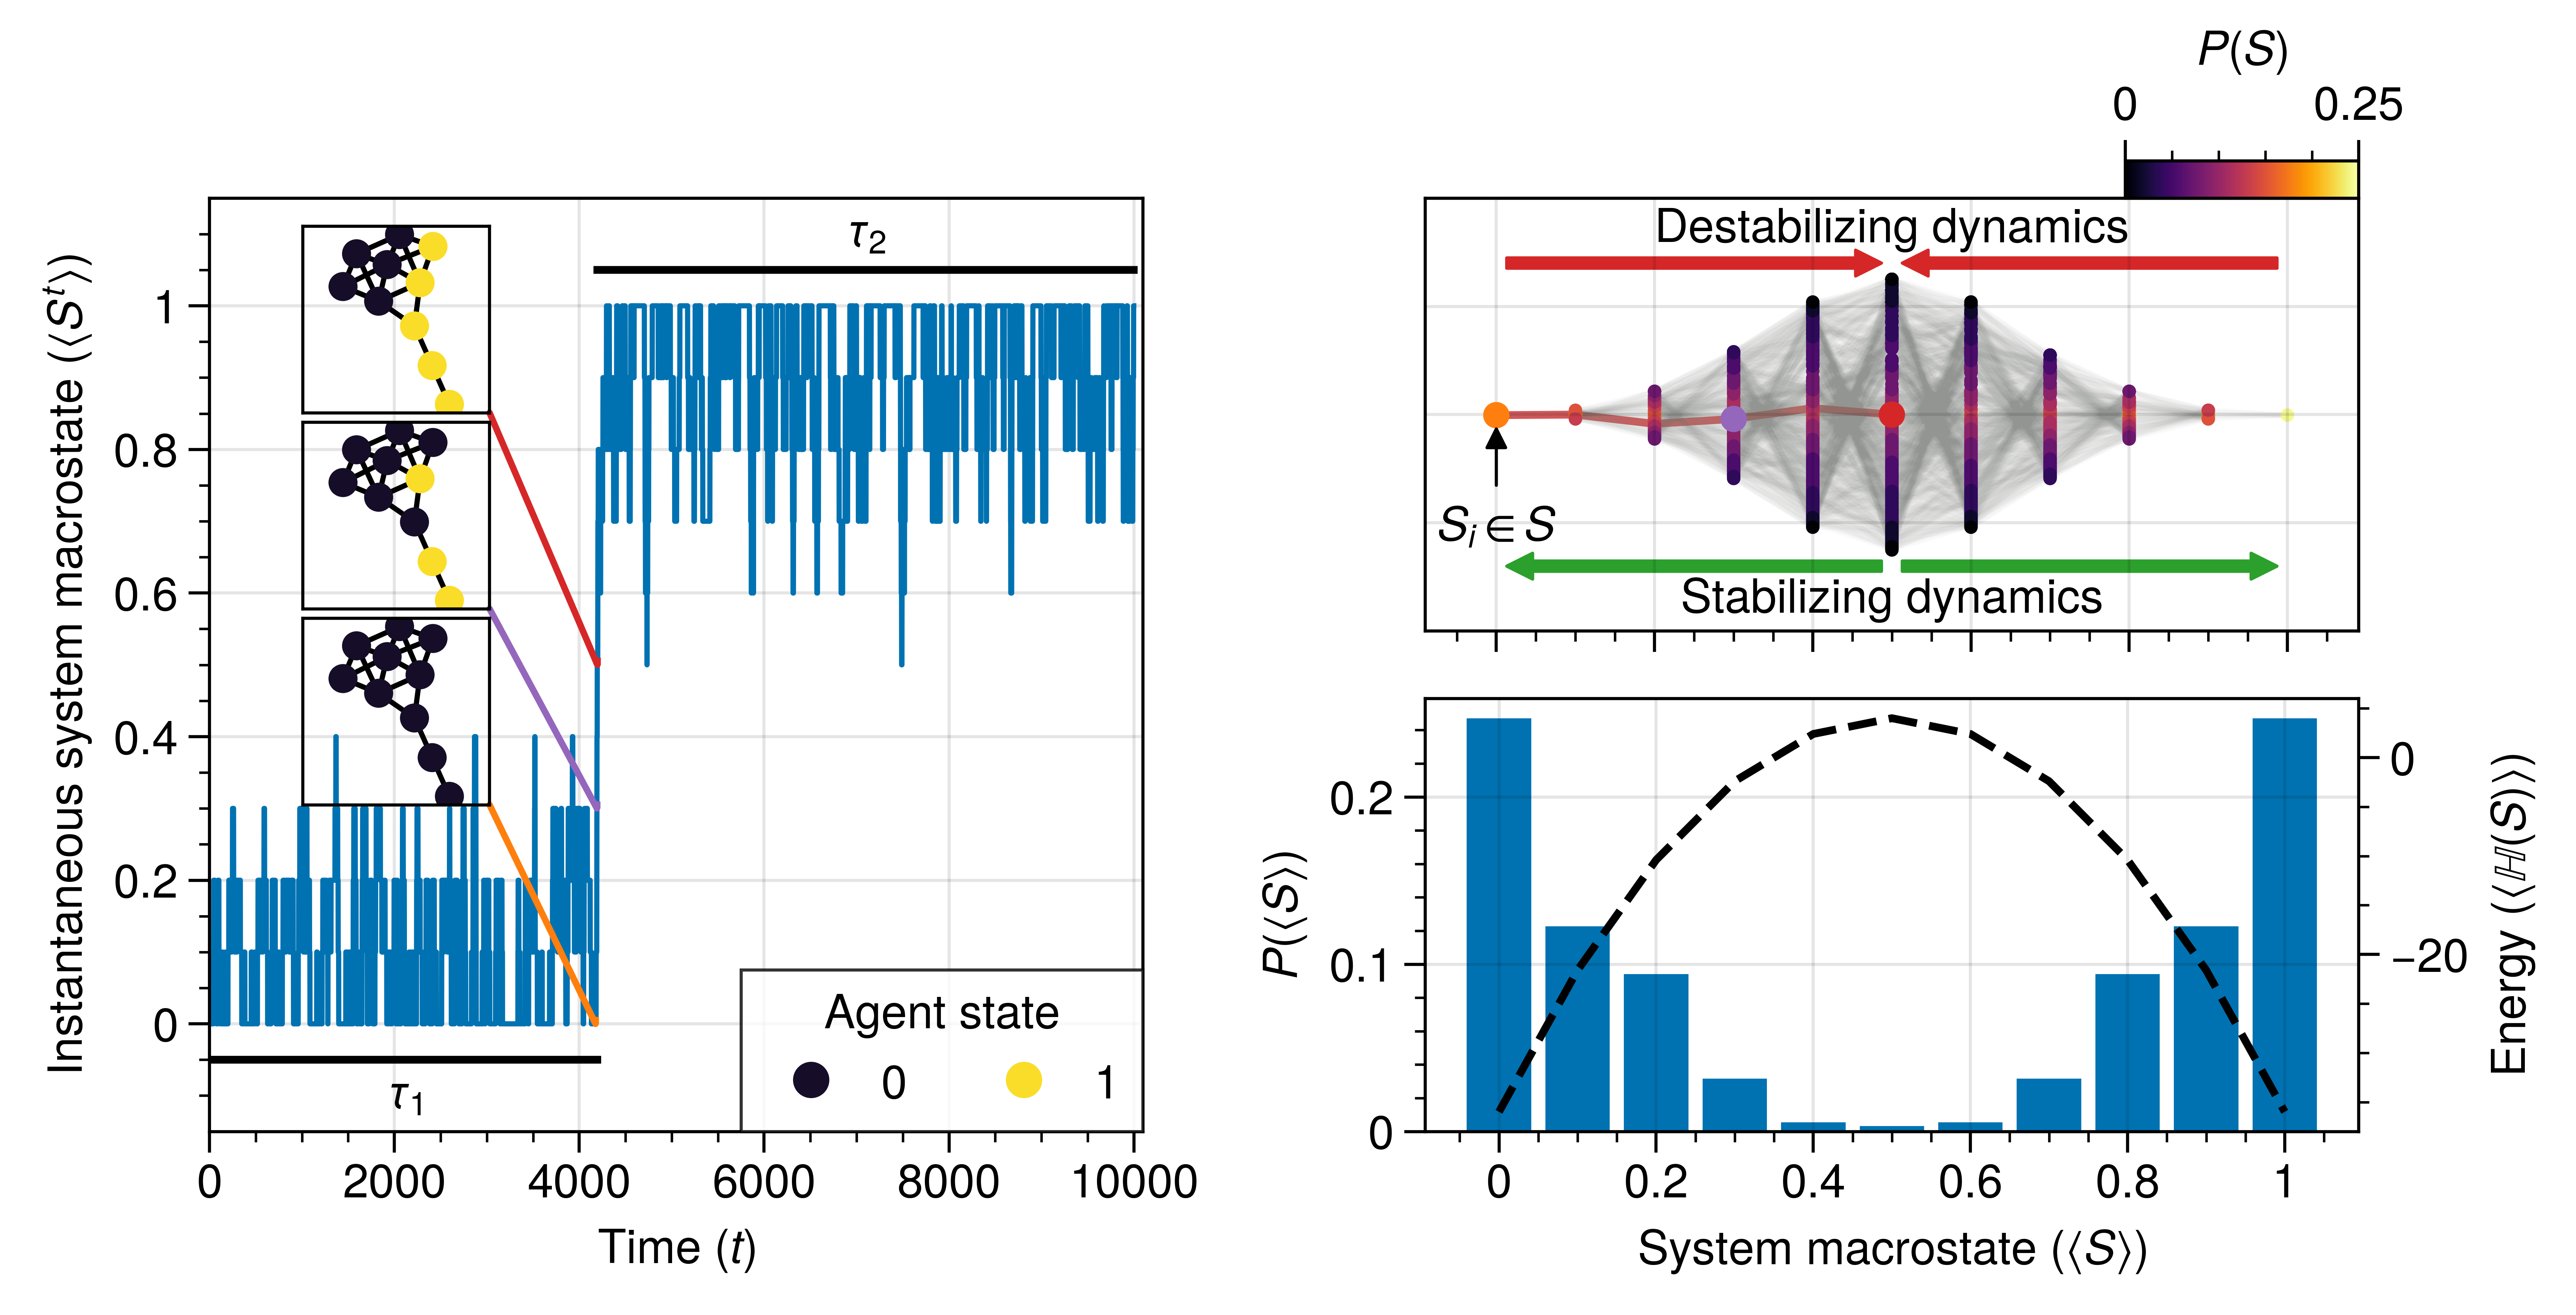
\includegraphics[width=.9\linewidth]{./figures/figure1_alt.pdf}
\caption{\label{fig:introduction}(a) A dynamical network governed by kinetic Ising dynamics produces multistable behavior. The metastable transitions occurs on a much shorter timescale than around one of the two metastable states (indicated by \(\tau\)). A typical trajectory is shown for a kite network for which each node is governed by the Ising dynamics with \(\beta \approx 0.534\). The panels show system configurations \(S_i \in S\) of as the system approaches the tipping point (orange to purple to red). For the system to transition between metastable point, it has to cross an energy barrier (inset right). (b) The dynamics of the system can be represented as a graph. Each node represents a system configuration \(S_i \in S\) such as depicted in (a). The probability for a particular system configuration \(P(S)\) is indicated with a color; some states are more likely than others. The trajectory from (a) is visualized. Dynamics that move towards the tipping point (midline) destabilize the system, whereas moving away from the tipping point are stabilizing dynamics. (c) The stationary distribution of the system is bistable. Transitions between the metastable states are infrequent and rare. For more information on numerical see \ref{sec:orgc2d2248}.}
\end{figure*}

\section{Results}
\label{sec:org6f0b033}
From  an information  perspective, the  contribution of  the
dynamics  of a  node  can be  quantified using  time-delayed
Shannon   information  \cite{Cover2005}.   Depending  on   the
connectivity of a node  in the system (\cref{fig:maj_flip}),
the  contribution  to  the  system  macrostate  will  differ
\cite{vanElteren2022,Quax2013}.  How  much the  future  system
state is affected by the node's current state is computed by
shared information with the node's current state \(s_i^{\tau}\) and
the  future system  state \(S^{\tau + t}\)  as the  integrated mutual
information

\begin{equation}
\label{eq:adj_imi}
\begin{split}
\mu(s_i) = \sum_{t = 0}^\infty (I(s_i^{\tau} : S^{\tau + t}) - \omega_{s_i}) \Delta t.
\end{split}
\end{equation}

Intuitively, \(\mu(s_i)\) represents the transient dynamics of
how  much the  influence of  a node  is ``remembered''  by the
system over  time \cite{vanElteren2022}.  It reflects  how the
effects of  local dynamics between nodes  percolates through
the  system  over  time.  As  the  system  chooses  it  next
metastable  state, the  system  macrostate  is dominated  by
transient dynamics.  The next tipping point  will be reached
on a  much longer timescale. Consequently,  \(\omega\) quantifies
the system  returning to a  stable system regime.  For nodes
with  fast  dynamics,  \(\mu(s_i)\)   is  generally  high  and
\(\omega_{s_i}\) would be generally low.

In  \cref{fig:introduction}{a-e} the  information flows  are
shown at different stages  in the metastable transition. The
metastable  transition  was  decomposed by  considering  the
local  information  flows  from  a  given  system  partition
\(S_{\gamma} = \{S' \subseteq  S | \langle S' \rangle = \gamma\}\) where  \(\gamma \in [0,1]\) is
the  fraction of  nodes  having state  +1.  This yields  the
conditional integrated mutual information as

\begin{equation}
\label{eq:adj_imi_conditional}
\begin{split}
\mu(s_i  | \langle  S \rangle) =  \sum_{t = 0}^\infty (I(s_i^{\tau} : S^{\tau + t} | \langle S^{\tau} \rangle) - \omega_{s_i}) \Delta t.
\end{split}
\end{equation}

By evolving all possible trajectories, the exact information
flows  are  computed  for \(t=500\)  steps.  Asymptotic  and
integrated mutual information are estimated using regression
(\ref{sec:orgc2d2248}).

\begin{figure*}[th]
\centering
\includegraphics[width=.9\linewidth]{./figures/figure2_alt.pdf}
\caption{\label{fig:kite_res}(a-e) Information flows as distance to tipping point. Far away from the tipping point most information processing occurs in low degree nodes (f,g). As the system moves towards the tipping point, the information flows increase and the information flows move towards higher degrees. (f) Integrated mutual information as function of distance to tipping point. The graphical inset plots show how noise in introduced far away from the tipping point in the tail of the kite graph. As the system approaches the tipping point, the local information dynamics move from the tail to the core of the kite. (g) A rise in asymptotic information indicates the system is close to a tipping point. At the tipping point, the decay maximizes as trajectories stabilize into one of the two metastable states.}
\end{figure*}

Two things are observed. First, the tipping point is reached
by a  domino effect where  low degree nodes flip  first, and
then causing  neighboring nodes to  flip. Far away  from the
tipping  point  (\cref{fig:kite_res}{a}),  nodes
with  lower  degree  have higher shared information  (higher
\(\mu(s_i |  \langle S \rangle)\)) than  higher degree nodes. This  can be
understood  by  considering  the   likelihood  of  the  node
flipping  as  a function  of  degree  and system  macrostate
(\cref{fig:maj_flip}).  Lower degree  nodes by
definition  have  fewer  constraints from  nearest  neighbor
interactions,  which makes  flipping  from  the majority  to
minority  states  more  likely  than  higher  degree  nodes.
Consequently, lower  degree nodes  drive the  system towards
the tipping point by injecting noise into the system. As the
system  is further  destabilized, the  flip probability  for
higher degree  nodes from  majority becomes more  likely and
the driver node changes to higher degree nodes closer to the
tipping point.

\begin{figure}[htbp]
\centering
\includegraphics[width=.9\linewidth]{./figures/butterfly_t=5.pdf}
\caption{\label{fig:butterfly}Shown are the conditional probability at time \(t=10\) relative to the tipping point. The shared information between the hub node 3 and the tail node 3 is shared is similar but importantly caused through different sources. The hub (node 3) has high certainty on that the system macrostate will be the same sign as its state. In contrast, node 8 has high certainty that the system macrostate will be opposite to its state at the tipping point. This is caused by the interaction between the network structure and the system dynamics whereby the most likely trajectories to the tipping point from the stable regime is mediated by the noise-induced dynamics from the tail to the core in the kite graph (see main text).}
\end{figure}

Second, an  increase in asymptotic behavior  correlates with
the  system  transitioning  from  one  metastable  point  to
another.  The asymptotic  information remains  low far  away
from the  tipping point, and monotonically  increases as the
system       approaches        the       tipping       point
\cref{fig:kite_res}{b,  c}). The  increase in  a
node's asymptotic information reflect how the system is more
likely to transition between metastable points. That is, the
system  either  relaxes  to  the  closest  ground  state  or
transitions  across   the  tipping   point  into   the  next
metastable state.  After such a transition,  the dynamics of
the nodes  slow down. That  is, all  but the nodes  with the
lowest  degrees are  locally frozen  as the  system dynamics
restabilizes after a noise-induced perturbation.

\begin{figure*}
\centering
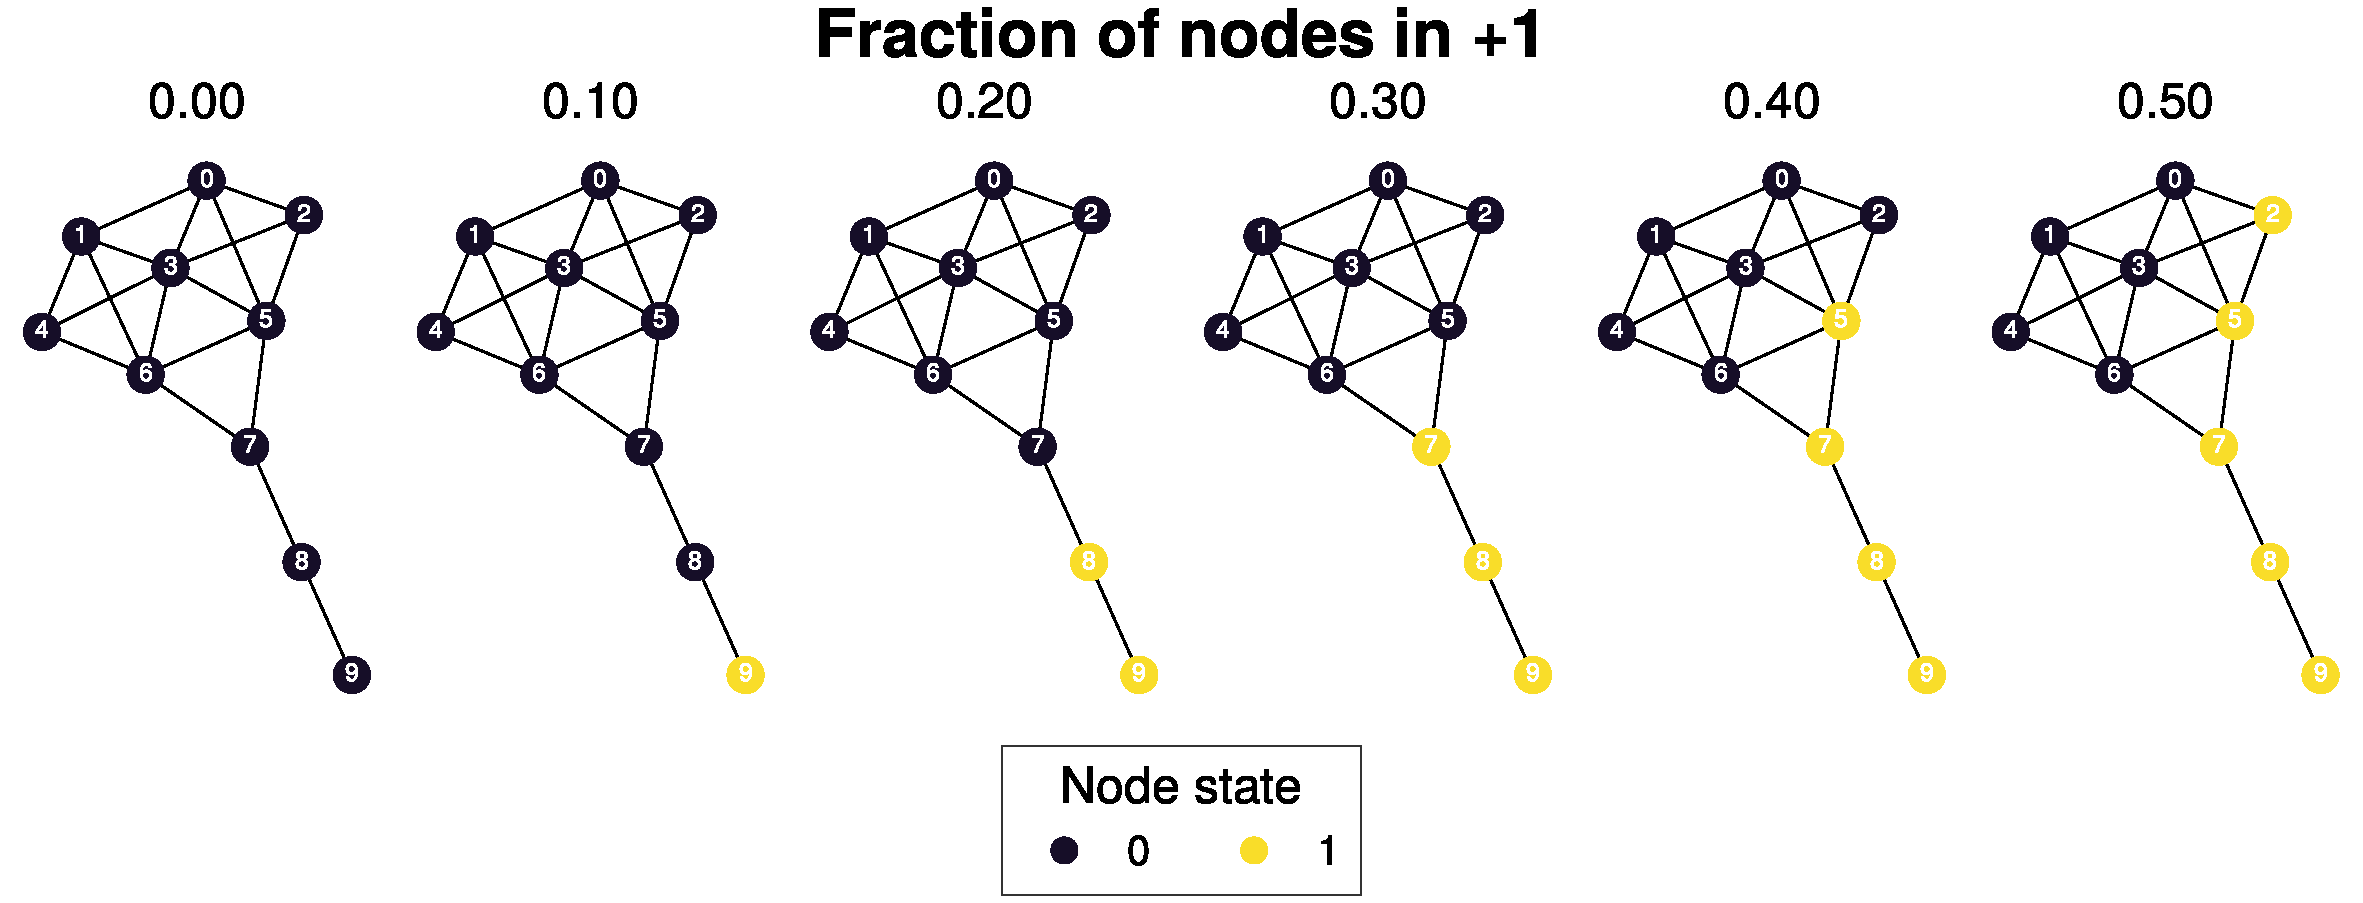
\includegraphics[width=.9\linewidth]{./figures/kite_maximized_trajectory_30230.pdf}
\caption{\label{fig:max_trajectory}The tipping point is initiated from the bottom up. Each node is colored according to state 0 (black) and state 1 (yellow) Shown is a trajectory towards the the tipping point that maximizes \(\sum_{{t=1}}^{{5}} \log p(S^{{t+1}} | S^t, S^0 =\{0\}, \langle S^5 \rangle ) = 0.5)\). As the system approaches the tipping point, low degree nodes flip first, and recruit ``higher'' degree nodes to further destabilize the system and push it towards a tipping point. In total 30240 trajectories that reach the tipping point in 5 steps, and there are 10 trajectories that have the same maximized values as the trajectory shown in this figure.}
\end{figure*}

\begin{figure*}
\centering
\includegraphics[width=.9\linewidth]{./figures/figure4_nudge=inf.pdf}
\caption{\label{fig:kite_noise}For a system to cross a tipping point two different types of nodes are identified. High degree nodes are essential for system to move from one metastable point to another. In contrast, low degree nodes are essential to propagate noise into the system. In (a) typical system trajectories are shown under pinning intervention on a node. Each color indicates a targeted intervention on the colors matching in (a). (b) The effect of intervention has a different effect depending on which node is targeted; Targeting a high degree node to the +0 state (e.g. node 3) prevents the system into tipping the opposite side of the pinning effect. In contrast, targeting a low degree node (e.g. 9) the system is still able to explore the full state space. Intermediate connected nodes (e.g. node 7, 8) removed merely nudges the system macrostate to one side, and increases the probability to remain in the +0 macrostate. In (b) +- 2 standard error of the mean are shown.}
\end{figure*}

To confirm  the mechanism underlying the  information flows,
trajectories   to   the   tipping   point   were   analyzed.
Trajectories were computed from the  ground state \(S = \{0,
\dots,   0\}\)  and   simulated   for   \(t=5\)  steps.   In
\cref{fig:max_trajectory}  a  trajectory
is shown that  maximizes reaching the tipping  point, i.e. a
path that maximizes

\begin{equation*}
\label{eq:max_trajectory}
\log P(S^{t + 1}|S^{t}, S^0 = \{0\}, \langle S^5 \rangle = 0.5).
\end{equation*}


These trajectories reveal how the information flows measured
in  \cref{fig:kite_res}{c}  are  caused  by  the
sequence  of flips  generated from  the ``tail''  in the  kite
graph.  These nodes  are  uniquely positioned  due to  their
higher  potential  to  pass  on  noise  to  their  neighbors
eventually causing a cascade of flips that reach the tipping
point.

Surprisingly, this effect is  not completely correlated with
degree. For example, consider node 8  and node 3. Node 8 has
degree 2  and has the highest  integrated mutual information
when 2  bits are flipped in  the system (\cref{fig:kite_res}
2nd column).  The dynamics for  node 8 for all  states where
\(\langle S  \rangle =  0.2\) (or  0.8 by symmetry)  indicate that  8 is
essential in  propagating the noise  generated by 9.  At the
tipping point,  node 8  shares the highest  information with
the system. In  contrast, node 3 which has degree  6 has low
shared information  prior to the tipping,  indicating that 3
is less involved with initializing the tipping point. At the
tipping point,  however, node 3  has high amounts  of shared
information with  the future system states,  similar to that
of node 8.

The  path analysis  reveal  that at  the  tipping point  the
system  can either  (a) move  from one  metastable point  to
another, or  (b) relax back  to the ground state  it evolved
from. The most likely paths  reaching the tipping point from
one of the ground state  results in a configuration in which
a  high  degree cluster  set  of  nodes  has to  flip  (e.g.
1,0,3,4,6 in \cref{fig:max_trajectory} at  \(\langle S \rangle = 0.5)\).
This trajectory  is less  likely than  essentially reversing
the path shown in  \cref{fig:max_trajectory}. Hence, most of
the tipping points  ``fail'' and relax back  to the metastable
ground state from which it evolved (\cref{fig:tip_suc}). If,
however, it does make the metastable transition to the other
side,  the ``tail''  in  the graph  remains  stable for  these
transitions,  yielding relative  high  correlation for  node
8, 9. The information flows reflect how certain a given node
is about  the future  system state,  e.g. \(H(S^{t + \tau}  | s_i^{t})\),
revealing  how  much  uncertainty  it  has  on  how  quickly
\(P(S^{t + \tau})\)  converges to  some  stable  trajectory around  a
future metastable state.

The information flows reflect the most probable trajectories
around the partition \(\langle S \rangle  = c\) and give unique insights
into the mechanism driving  the tipping behavior. Over time,
local clusters  will stabilize.  Some nodes  will experience
more  ``frustration'' than  others. In  other words,  the node
will tend to change state more  as the effect of a node flip
percolates through the system.  For example, the light green
and yellow node has  the lowest asymptotic information while
still  having   a  relatively   high  degree.   These  nodes
experience more frustration as  it they attempt to reconcile
with the states of the nearest neighbors.

The  cascade  of  flips  is  further  studied  using  causal
interventions (\cref{fig:kite_noise}). By  pinning each node
state  to +0  in  separate simulations,  the  effect on  the
occurrence of  tipping points is studied.  The interventions
highlight two distinct roles for the metastable transitions.
Intervention on low degree nodes removes fluctuations in the
system macrostate +0 but increases the fluctuations when the
system  reaches  the  macrostate  +1.  The  effect  is  most
prominent    for    node    9    which    has    degree    1
(\cref{fig:kite_noise}{c}); interventions  on node  9 yields
the   lowest  time   spent  in   the  +0   metastable  state
(\cref{fig:kite_noise}{a}),  and the  highest time  spent in
the  +1  macrostate  relative   to  interventions  on  other
nodes(\cref{fig:kite_noise}{b}).  Notable,   the  number  of
tipping transitions  is the  least affected by  lower degree
nodes. In contrast,  high degree nodes seem  to be essential
for the tipping  behavior to endure; lower  degree nodes are
necessary to  destabilize the system, but  the higher degree
nodes have to flip in order  for the new metastable state to
endure.  This can  be  seen  by the  time  spent  in the  +1
macrostate: interventions on a  hub node has increased white
noise compared  to control  conditions in the  +0 macrostate
(\cref{fig:kite_noise}{a}).  This  indicates that  noise  is
propagated and nodes are  flipped towards the tipping point,
but  are less  likely to  cross the  tipping point.  This is
further strengthened  by the  reduced time  spent in  the +1
macrostate as a function of degree \cref{fig:kite_noise}{b}.


\begin{figure}[htbp]
\centering
\includegraphics[width=.9\linewidth]{./figures/tipping_success.pdf}
\caption{\label{fig:tip_suc}Successful metastable transitions are affected by network structure. Successful metastable transitions are those for which the sign of the macrostate is not the same prior and after the tipping point, e.g. the system going from the +0 macrostate side to the +1 macrostate side or vice versa. Shown here are the number of successful metastable transitions for \cref{fig:kite_noise} under control and pinning interventions on the nodes in the kite graph.}
\end{figure}

\section{Discussion}
\label{sec:org389dbab}
Understanding how  metastable transitions occur may  help in
understanding  how, for  example,  a pandemic  occurs, or  a
system undergoes critical failure.  In this paper, dynamical
networks governed  by the Boltzmann-Gibbs  distribution were
used   to  study   how  endogenously   generated  metastable
transitions    occur.   The    external   noise    parameter
(temperature) was fixed such that the statistical complexity
of  the  system behavior  was  maximized  (see \ref{sec:orgc2d2248}).

The results show that in the network two distinct node types
could  be identified:  \emph{initiator}  and \emph{stabilizer}  nodes.
Initiator  nodes  are  essential  early  in  the  metastable
transition. Due to their high degree of freedom, these nodes
are more  effected by  external noise. They  are instigators
and inject noise into  the system, destabilizing more stable
nodes. In  contrast, stabilizer  nodes, have high  degree of
freedom and require more energy to change state. These nodes
are essential for the  metastable behavior as they stabilize
the system  macrostate. During  the metastable  transition a
domino sequence of  node state changes are  propagated in an
ordered sequence towards the tipping point.

This  domino effect  was  revealed  through two  information
features unvealing an \emph{information cascade} underpinning the
trajectories towards the tipping point.

Integrated  mutual  information   captured  how  short-lived
correlations are passed  on from the initator  nodes. In the
stable regime (close  to the ground state)  low degree nodes
drive the system dynamics.  Low degree nodes destabilize the
system, pushing the  system closer to the  tipping point. In
most cases, the initiator nodes will fail in propagating the
noise to  their neighbors.  On rare occasions,  however, the
cascade  is propagated  progressively  from  low degree,  to
higher  and higher  degree. A  similar domino  mechanism was
recently        found        in       climate        science
\cite{Wunderling2020,Wunderling2021}.      Wunderling      and
colleagues  provided  a  simplified  model  of  the  climate
system, analyzing  how various components contribute  to the
stability  of  the  climate. They  found  that  interactions
generally  stabilize the  system  dynamics.  If, however,  a
metastable transitions was initialized, noise was propagated
through  a  similar  mechanism   found  here.  That  is,  an
``initializer'' node propagated noise through the system which
created a domino effect  that percolated through the system.
The results  from this  study mirrors these  conclusions and
provides  a  model-free  language to  express  these  domino
effects.

An increase in asymptotic  information forms an indicator of
how close  the system is  to a  tipping point. Close  to the
ground state, the asymptotic  information is low, reflecting
how transient noise perturbations  are not amplified and the
system macrostate relaxes  back to the ground  state. As the
system   approaches  the   tipping  point,   the  asymptotic
information increases.  As the distance to  the ground state
increases, the  system is more likely  to transition between
metastable  states. After  the transition,  there remains  a
longer term correlation. Asymptotic information reflects the
long(er)  timescale  dynamics  of the  system.  This  ``rest''
information  peaks  at  the  tipping point,  as  the  system
chooses its next state.

The  information   viewpoint  uniquely  reveals   a  complex
mechanism of  interaction underlying the  system macrostate.
It reduced  the complexity  of high  dimensional probability
distribution in  human-interpretable terms.  Furthermore, it
revealed   how  some   nodes   may   have  high   predictive
information, which  is hard to infer  from their interaction
structure alone \cref{fig:butterfly}. Integrated information
and asymptotic information jointly readout the separation of
fast-time   scale   dynamics    that   tend   to   stabilize
noise-induced   dynamics,   and  slow   timescale   dynamics
indicating  a  metastable   transition.  Importantly,  these
measures can be directly computed on data.

It is important to emphasize,  that for the ergodic dynamics
considered here,  the information should decay  back to zero
due  to  the   data-processing  inequality.  The  asymptotic
information approximates  this decay as an  apparent offset.
This  offset   appears  as   the  transition   time  between
metastable states is on much  longer timescale than the fast
dynamics   measured   by   integrated   mutual   information
(\cref{fig:introduction}{c}).

\section{Conclusions}
\label{sec:org7971cd6}
The information theoretic approach offers an alternative view to
understand \emph{how} metastable transitions occur in dynamical networks. Two
information features were introduced that decompose the metastable
transition in terms sources of high information processing (integrated
mutual information) and distance of the system to the tipping point
(asymptotic information). A domino effect was revealed, whereby low
degree nodes initiate the tipping point, making it more likely for
higher degree nodes to tip. On the tipping point, long-term correlations
stabilizes the system inside the new metastable state. Importantly, the
information perspective allows for estimating integrated mutual
information directly estimated from data without knowing the mechanisms
that drive the tipping behavior. The results highlight how short-lived
correlations are essential to initiate the information cascade for
crossing a tipping point.

\section{Limitations}
\label{sec:org26f073f}
Integrated mutual  information was  computed based  on exact
information  flows. This  means that  for binary  systems it
requires  to  compute a  transfer  matrix  on the  order  of
\(2^{|S|} \times 2^{|S|}\). This  reduced the present analysis to
smaller  graphs. It  would  be possible  to use  Monte-Carlo
methods   to  estimate   the  information   flows.  However,
\(I(s_i : S^t)\) remains expensive to compute.

In addition, the decomposition  of the metastable transition
depends  on the  partition of  the state  space. Information
flows are  in essence statistical dependencies  among random
variables. Here,  the effect  of how  the tipping  point was
reached was studied by partition the average system state in
terms of  number of bits flipped.  This partitioning assumes
that the majority  of states prior to the  tipping point are
reached by having fraction \(c  \in [0, 1]\) bits flipped. The
contribution  of  each  system  state  over  time,  however,
reflects a  distribution of  different states;  reaching the
tipping  point from  the  ground  state 0,  can  be done  at
\(t-2\) prior to tipping by either remaining in 0.4 bits, or
transitioning from 0.3 bits flipped to 0.4 and eventually to
0.5 in  2 time steps. Additionally,  analyses by numerically
estimating  tipping points.  The effect  of this  additional
path  showed  marginal  effects  on  the  integrated  mutual
information and asymptotic information.

Information flows  conditioned on a  partition is a  form of
conditional   mutual   information  \cite{James2016a}.   Prior
results   showed  that   conditional  information   produces
synergy, i.e. information that is  only present in the joint
of all variables but cannot be found in any of the subset of
each variable.  Unfortunately, there is no  generally agreed
upon    definition    on     how    to    measure    synergy
\cite{Beer2015,Kolchinsky2022}  and different  estimates exist
that may  over or  underestimate the synergetic  effects. By
partitioning one can create synergy as for a given partition
each spin  has some  additional information about  the other
spins. For example, by taking the states such that \(\langle S \rangle =
0.1\),  each spin  ``knows'' that  the average  of the  system
equals 0.1. This creates shared information among the spins.
Analyses  were  performed  to  estimate  synergy  using  the
redundancy  estimation  \(I_{min}\)\cite{Williams2010}.  Using
this  approach, no  synergy was  measured that  affected the
outcome of this study. However, it should be emphasized that
synergetic effects  may influence the  causal interpretation
of the approach presented here.

Note that  for these  simulations the Krackhardt  kite graph
was used as it shows a  rich variation in the degrees of the
nodes  given   the  small   network  size.   Crucially,  the
information theory  approach is  model free  and generalizes
readily   to   systems   with  other   networks   structures
\cref{fig:other_systems}.

A  general class  of  systems was  studied  governed by  the
Boltzmann-Gibbs  distribution.  For practical  purposes  the
kinetic Ising model  was only tested, but  we speculate that
the  results should  hold (in  principle) for  other systems
dictated by  the Boltzmann-Gibbs distribution. We  leave the
extension for other system Hamiltonians up to future work.

\section{Acknowledgments}
\label{sec:orgf30530a}
I would like to thank Fiona Lippert, and Jair Lenssen for providing
insights and feedback in various ideas present in this paper. This
research is supported by grant Hyperion 2454972 of the Dutch National
Police.

\section{References}
\label{sec:org26fe258}
\section{Appendix}
\label{sec:org854db8e}
\subsection{Background, scope \& innovation}
\label{sec:orgd888f8c}
Noise  induced transitions  produces may  produce metastable
behavior that is fundamental  for the functioning of complex
dynamical  systems.  For  example, in  neural  systems,  the
presence   of   noise   increase   information   processing.
Similarly, the  relation between glacial ice  ages and earth
eccentricity has  been shown  to have a  strong correlation.
Metastability manifests itself by means of noise that can be
of two  kinds \cite{Forgoston2018}. External  noise originates
form   events   outside   the   internal   system   dynamics
\cite{Calim2021,Czaplicka2013a}.    Examples    include    the
influence of climate effects,  population growth or a random
noise  source  on a  transmission  line.  External noise  is
commonly modeled  by replacing an external  control or order
parameter  by  a  stochastic  process.  Internal  noise,  in
contrast, is inherent to the  system itself and is caused by
random  interactions   of  elements  of  the   system,  e.g.
individuals  in  a  population,  or  molecules  in  chemical
processes.  Both  types  of noise  can  generate  metastable
transitions between one metastable state to another. In this
paper, the metastable behavior  is studied of internal noise
in complex dynamical networks  governed by the kinetic Ising
dynamics.

The ubiquity of multistability  in complex systems calls for
a   general  framework   to   understand  \emph{how}   metastable
transitions occur.  The diversity of complex  systems can be
captured by an interaction  networks that dynamically evolve
over  time. These  dynamics can  be seen  as a  distributive
network of  computational units, where each  unit or element
of the  interaction network  changes it  state based  on the
input it  gets from its local  neighborhood. Lizier proposed
that these proposed that  the dynamic interaction of complex
systems  can  be  understood   by  their  local  information
processing \cite{Lizier2008,Lizier2013,Lizier2018}. Instead of
describing  the dynamics  of the  system in  terms of  their
domain  knowledge such  as  voltage  over distance,  disease
spreading rate,  or climate  conditions, one  can understand
the  dynamics in  terms  of the  \emph{information dynamics}.  In
particular, the  field of information dynamics  is concerned
with describing  the system  behavior along its  capacity to
store   information,   transmit  information,   and   modify
information.  By abstracting  away the  domain details  of a
system  and recasting  the dynamics  in terms  of \emph{how}  the
system  computes  its  next   state,  one  can  capture  the
intrinsic computation a system performs. The system behavior
is  encoded in  terms of  probability, and  the relationship
among  these variables  are explored  using the  language of
information theory \cite{Quax2017}.

Information theory offers profound benefits over traditional
methods used in metastable analysis as the methods developed
are model-free, can capture non-linear relationships, can be
used for both discrete and  continuous variables, and can be
estimated   directly  from   data  \cite{Cover2005}.   Shannon
information measures  such as mutual information  and Fisher
information can  be used to  study how much  information the
system   dynamics   share   with   the   control   parameter
\cite{Nicolis2016,Lizier2010}.

Past work  on information  flows and  metastable transitions
focus  on methods  to detect  the onset  of a  tipping point
\cite{Scheffer2009,Prokopenko2011,Scheffer2001}.    It   often
centers around  an observation that the  system's ability to
absorb noise  reduces prior  to the  system going  through a
critical point. This critical  slowing down, can be captured
as  a statistical  signature  where  the Fisher  information
peaks \cite{Eason2014}.  However, these  methods traditionally
use  some  form  of  control parameter  driving  the  system
towards  or  away from  a  critical  point. Most  real-world
system lack such an  explicit control parameter and requires
different  methods. Furthermore,  detecting a  tipping point
does not  necessarily lead to further  understanding how the
tipping point  was created. For  example, for a  finite size
Ising model,  the system produces bistable  behavior. As one
increases  the   noise  parameter,  the   bistable  behavior
disappears. The  increase in  noise effectively  changes the
energy landscape, but little information is gained as to how
initially the metastable behavior occured.

In this work,  a novel approach using  information theory is
explored  to study  metastable behavior.  In particular,  we
focus  on  the  information  storage capacity  of  a  node's
ability  to   predict  the   future  state  of   the  system
\cite{Lizier2013}.  Two information  features are  introduced.
Integrated mutual information measure predictive information
of  a  node   on  the  future  of   the  system.  Asymptotic
information measures the long timescale memory capacity of a
node. These  measures differ from previous  information such
as  transfer  entropy   \cite{Schreiber},  conditional  mutual
information under causal intervention \cite{Ay2008}, causation
entropy \cite{Runge2019}, time-delayed variants \cite{Li2008} in
that  these  methods  are  used to  infer  the  transfer  of
information between sets of nodes by possible correcting for
a third  variable. Here, instead,  we aim to  understand how
the  elements in  the system  contribute to  the macroscopic
properties of the system. It  is important to emphasize that
information  flows are  not  directly  comparable to  causal
flows \cite{James2016}. A  rule of thumb is  that causal flows
focuses  on  micro-level   dynamics  (\(X\)  causes  \(Y\)),
whereas information flows focus on the predictive aspects, a
holistic  view of  emergent  structures \cite{Lizier2013}.  In
this sense,  this work is similar  to predictive information
\cite{Bialek1999} where predictive  information of some system
\(S\) is projected onto its  consistent elements \(s_i \in S\)
and computed as a function of time \(t\).

\subsection{Methods and definitions}
\label{sec:orgc2d2248}
\subsubsection{Model}
\label{sec:org5382bb5}
To  study metastable  behavior, we  consider a  system as  a
collection of  random variables \(S =  \{s_1, \dots, s_n\}\)
governed by the Boltzmann-Gibbs distribution

\[P(S)    =     \frac{1}{Z}    \exp(- \beta \mathcal{H}(S) ),\]

where is  the inverse temperature \(\beta  = \frac{1}{T}\) which
control the  noise in the system,  \(\mathcal{H}(S)\) is the
system Hamiltonian which encodes the node-node dynamics. The
choice of the  energy function dictates what  kind of system
behavior we observe. Here, we focus on arguable the simplest
models  that shows  metastable behavior:  the kinetic  Ising
model, and the Susceptible-Infected-Susceptible model.

Temporal  dynamics  are  simulated  using  Glauber  dynamics
sampling.  In each  discrete time  step a  spin is  randomly
chosen  and  a   new  state  \(X'\in  S\)   is  accepted  with
probability

\begin{equation}
\label{eq:glauber}
\begin{split}
 p(  \text{accept} X'  ) =  \frac{1}{1 +
\exp(-\beta   \Delta  E)},
\end{split}
\end{equation}

where  \(\Delta E  =  \mathcal{H}(X') -  \mathcal{H}(X)\) is  the
energy difference  between the  current state \(X\)  and the
proposed state \(X'\).

\subsubsection{Kinetic Ising model}
\label{sec:orgb324012}
The  traditional Ising  model  was  originally developed  to
study ferromagnetism, and is  considered one of the simplest
models that generate complex behavior.  It consists of a set
of binary distributed spins \(S = \{s_1, \dots s_n\}\). Each
spin contains energy given by the Hamiltonian

\begin{equation}
\label{eq:energy}
\begin{split}
\mathcal{H}(S) = -\sum_{i,j} J_{ij} s_{i} s_{j} - h_{i} s_{i}.
\end{split}
\end{equation}

where  \(J_{ij}\) is  the  interaction energy  of the  spins
\(s_i, s_j\).

The  interaction energy  effectively encodes  the underlying
network   structure  of   the   system.  Different   network
structures are used in this study to provide a comprehensive
numerical overview of the relation between network structure
and  information   flows  (see  \ref{sec:orgc2d2248}).  The
interaction energy  \(J_{ij}\) is set  to 1 if  a connection
exists in the network.

For sufficiently  low noise  (temperature), the  Ising model
shows   metastable  behavior   (\cref{fig:introduction}{c}).
Here,  we aim  to  study  \emph{how} the  system  goes through  a
tipping point by tracking the information flow per node with
the entire system state.

\subsection{Information flow on complex networks}
\label{sec:org3d3e541}
Informally, the information flows measures the statistical coherence
between two random variables \(X\) and \(Y\) over time such that the
present information in \(Y\) cannot be explained by the past of \(Y\)
but rather by the past of \(X\). Estimating information flow is
inherently difficult due to the presence of confounding which potential
traps the interpretation in the ``correlation does not equal causation''.
Under some context, however, information flow can be interpreted as
causal \cite{vanElteren2022}. Let \(S=\{s_1, \dots, s_n\}\) be a random
process, and \(S^t\) represent the state of the random process at some
time \(t\). The information present in \(S\) is given as the Shannon
entropy

\begin{equation}
\label{eq:entropy}
\begin{split}
H(S) = \sum_{x \in S} p(x) \log p(x)
\end{split}
\end{equation}


where \(\log\) is base 2 unless otherwise stated, and \(p(x)\) is used
as a short-hand for \(p(S  = x)\). Shannon entropy captures the
uncertainty of a random variable; it can be understood as the number of
yes/no questions needed to determine the state of \(S\). This measure of
uncertainty naturally extends to two variables with Shannon mutual
information. Let \(s_i\) be an element of the state of \(S\), then the
Shannon mutual information \(I(S; s_i)\) is given as

\begin{equation}
\label{eq:mi}
\begin{split}
I(S; s_i) &= \sum_{S_i\in S, s' \in s_i} p(S_i,s') \log \frac{p(S_i,s')}{p(S_i)p(s')}\\
          &= H(S) - H(S | s_i)
\end{split}
\end{equation}


Shannon mutual information can be interpreted as the uncertainty
reduction of \(S\) after knowing the state of \(s_i\). Consequently, it
encodes how much statistical coherence \(s_i\) and \(S\) share. Shannon
mutual information can be measured over time to encode how much
\emph{information} (in bits) flows from state \(s_i\) to \(S^{t}\)

\begin{equation}
\label{eq:flow}
\begin{split}
I(S^t; s_i) = H(S^t) - H(S^t | s_i).
\end{split}
\end{equation}

Prior results showed that the nodes with the highest causal importance
are those nodes that have the highest information flow (i.e. maximize
\ref{eq:flow}) \cite{vanElteren2022}. Intuitively, the nodes
for which the future system ``remembers'' information from a node in the
past, is the one that ``drives'' the system dynamics. Formally, these
driver nodes can be identified by computing the total information flow
between \(S^t\) and \(s_i\) can be captured with the integrated mutual
information \cite{vanElteren2021}

\begin{equation}
\label{eq:imi}
\begin{split}
\mu(s_i) = \sum_{\tau = 0}^{\infty} I(s_{i}^{t-\tau} ; S^t).
\end{split}
\end{equation}

The driver nodes are the nodes that maximize \ref{eq:imi}. Note
that in \cite{vanElteren2022} \(I(S  :  s_i^{t})\) was considered.
Here, information flows are computed out-of-equilibrium with symmetry
breaking. That is, the system dynamics are evolved by starting the
system at a distance from the tipping point and evolving it
out-of-equilibrium. This causes \(I(s_i^t : S)\) to not follow the data
processing inequality as information may flow back into a node. The
choice for computing \(I(s_i^t :  S)\) over \(I(s_i  : S^t)\) was done
for computational feasibility in \cite{vanElteren2022}. Furthermore,
the data processing inequality was not violated when considered the
system without symmetry breaking. For \ref{eq:flow} the data
processing inequality is guaranteed, however it is computationally more
challenging to compute (see \hyperref[sec:org26f073f]{5}).

\subsection{Noise matching procedure}
\label{sec:org11ee4e3}
The Boltzmann-Gibbs distribution is parameterized by noise factor
\(\beta =  \frac{1}{kT}\) where \(T\) is the temperature and \(k\) is
the Boltzmann constant. For high \(\beta\) values metastable behavior
occurs in the kinetic Ising model. The temperature was chosen such that
the statistical complexity \cite{Lopez-Ruiz1995a} was maximized. The
statistical complexity \(C\) is computed as

\[C = \bar H(S) D(S),\]

where \(\bar H(S) = \frac{H(s)}{-\log_2(|S|)}\) is the system entropy,
and \(D(S)\) measures the distance to disequilibrium

\[D(S) = \sum_i (p(S_i) - \frac{1}{|S|})^2.\]

A typical statistical complexity curve is seen in
\cref{fig:stat_compl}. The noise parameter \(\beta\) is set such that
it maximizes the statistical complexity using numerical optimization
(COBYLA method in scipy's \texttt{optimize.minimize} module)
\cite{Virtanen2020}.

\begin{figure}[htbp]
\centering
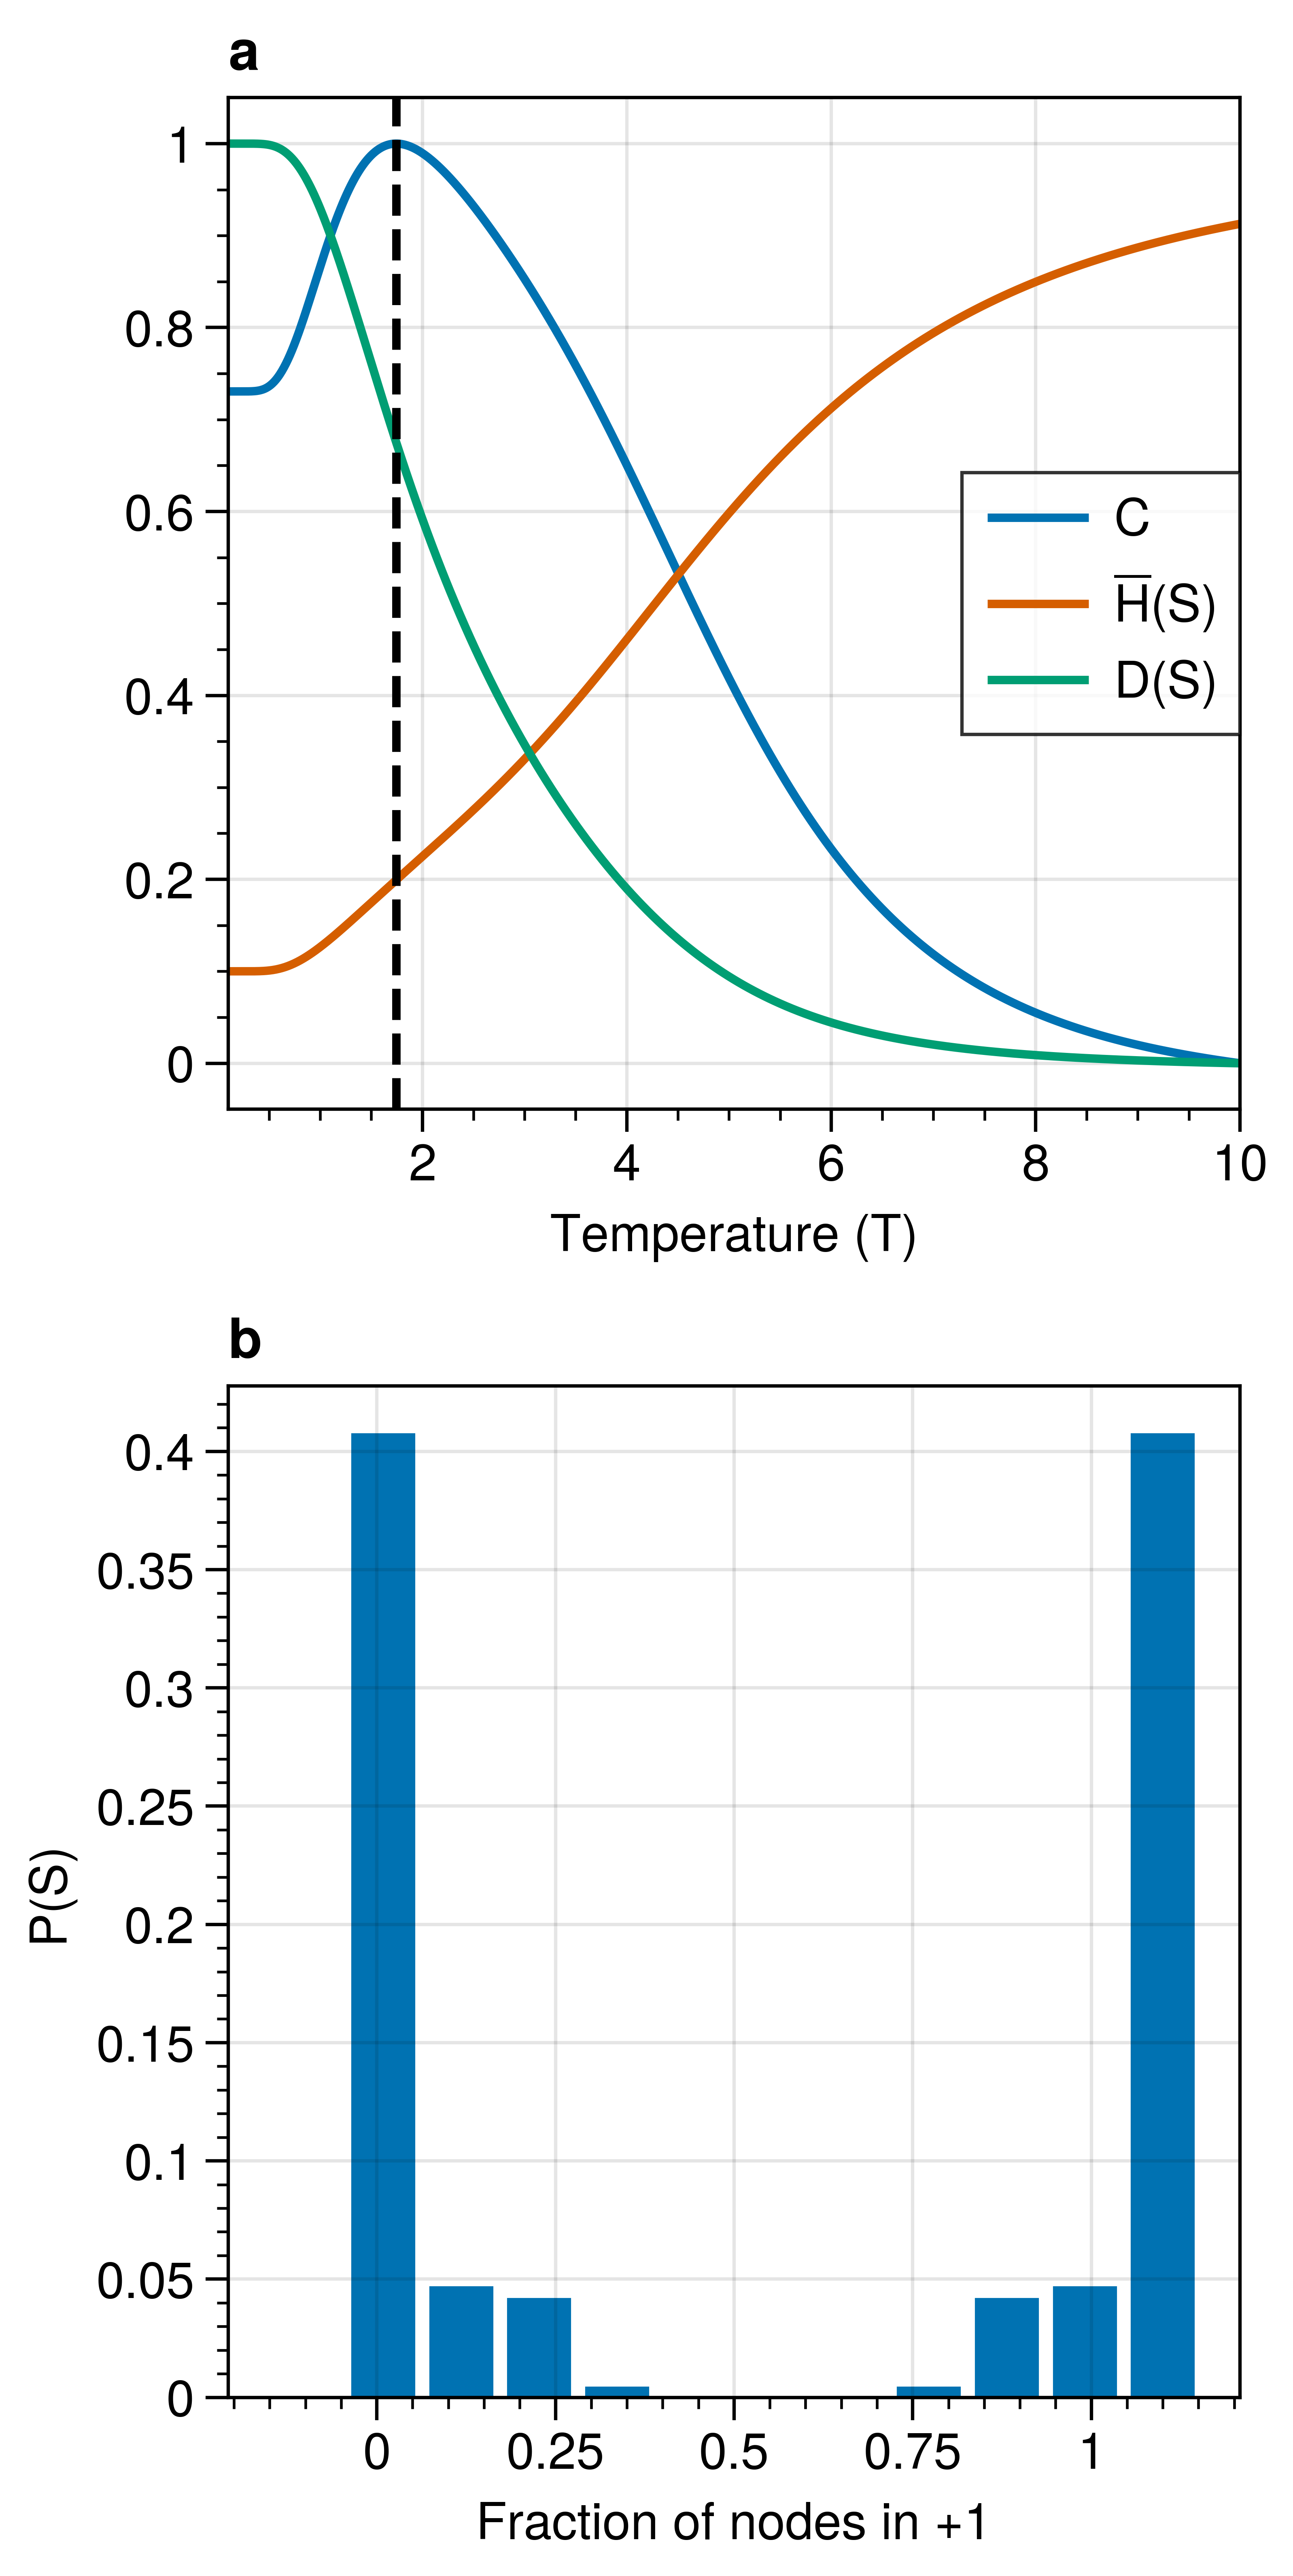
\includegraphics[width=.9\linewidth]{./figures/exact_kite_dyn=ising_beta=0.5732374683235916_T=200_statistical_complexity.png}
\caption{\label{fig:stat_compl}(a) Statistical complexity (\(C\)), normalized system entropy (\(H(S)\)) and disequilibrium (\(D(S)\)) as a function of the temperature (\(T = \frac{1}{\beta}\)) for Krackhardt kite graph. The noise parameter was set such that it maximizes the statistical complexity (vertical black line). The values are normalized between [0,1] for aesthetic purposes. (b) State distribution \(P(S)\) for temperature that maximizes the statistical complexity in (a) as a function of nodes in state +1.}
\end{figure}

\subsection{Exact information flows \(I(s_i^{\tau} ; S^{t + \tau})\)}
\label{sec:org59af222}
In  order  to  compute  \(I(s_i^{\tau}  :  S^{\tau + t})\),  the
conditional  distribution \(p(S^{\tau  +  t}  | s_i^{\tau})\)  and
\(p(S^{\tau + t})\) needs to  be computed. For Glauber dynamics,
the system  \(S\) transitions into \(S'\)  by considering to
flips  by randomly  choosing  node  \(s_i\). The  transition
matrix \(P(S^t |  s_i) = \textbf{P}\) can  be constructed by
computing each entry \(p_{ij}\) as

\[\label{eq:glauber}
\begin{split}
p_{ij, i \neq j} &= \frac{1}{|S|} \frac{1}{ 1 + \exp (-\Delta E) }\\
p_{ii} &= 1 - \sum_{j, j \neq i} P_{ij},
\end{split}\]

where \(\Delta E =  \mathcal{H}(S_j) - \mathcal{H}(S_j)\) encodes
the energy difference of moving from \(S_i\) to \(S_j\). The
state to  state transition \(\textbf{P}\) matrix  will be of
size  \(2^{|S|}  \times  2^{|S|} \times  |\mathcal{A}_{s_i}|\),  where
\(|\mathcal{A}_{s_i}|\)  is  the  size of  the  alphabet  of
\(s_i\),  which becomes  computationally intractable  due to
its  exponential growth  with the  system size  \(|S|\). The
exact information  flows can then be  computed by evaluating
\(p(S^t  |  s_i)\)  out  of equilibrium  by  evaluating  all
\(S^t\)  for   all  possible   node  states   \(s_i\)  where
\(p(S^t)\) is computed as

\[p(S^{\tau + t}) = \sum_{s_i} p(S^{\tau + t} | s_i^{\tau} ) p(s_i^{\tau}).\]

\subsection{Noise estimation procedure}
\label{sec:orgc093508}
Tipping point behavior under intervention was quantified by evaluating
the level of noise on both side of the tipping point. Let \(T1\)
represent the ground state where all spins are 0, \(T2\) where all
spins, and the tipping point \(TP\) is where the instantaneous
macrostate \(M(S^t) = 0.5\). Fluctuations of the system macrostate was
evaluated by analyzing the second moment above and below the tipping
point. This was achieved by numerically simulating the system
trajectories under 6 different seeds for \(t = 1e6\) time-steps. The
data was split between two sets (above and below the tipping point) and
the noise \(\eta\) was computed as

\begin{equation*}
\label{eq:noise}
\begin{split}
\eta = \frac{1}{\alpha^2 |S_{w}|}  \sum_w {S_w^t}^2,
\end{split}
\end{equation*}


where \(w \in \{\langle S \rangle < 0.5,\langle S \rangle > 0.5\}\), and

\begin{equation}
\label{eq:noise_estimation}
S_{w}^{t} = \Bigl\{\begin{aligned}
    S^t & \textrm{ if } S^t < 0.5 \\
    1 - S^t & \textrm{ if } S^t > 0.5
    \end{aligned}
\end{equation}

is the instantaneous system trajectory for the system macrostate above
or below the tipping point value. The factor \(\alpha\) corrects for the
reduced range the system macrostate has under interventions. For example
pinning a node \(s_i\) to state +0, reduces the maximum possible
macrostate to \(1 - \frac{1}{n}\) where \(n\) is the size of the system.
The correction factor \(\alpha\) is set such that for an intervention on
+0 for a particular node, the range \(S_{\langle S \rangle > 0.5}\)
alpha is set to \(\frac{n}{2} - \frac{1}{n}\).

\subsection{Switch susceptibility as a function of degree}
\label{sec:org009e10c}
First, we investigate the susceptibility of a spin as a function of its
degree. The susceptibility of a spin switching its state is a function
both of the system temperature \(T\) and the system dynamics. The system
dynamics would contribute to the susceptibility through the underlying
network structure either directly or indirectly. The network structure
produces local correlations which affects the switch probability for a
given spin.

As an initial approximation, we consider the susceptibility of a target
spin \(s_i\) to flip from a majority state to a minority state given the
state of its neighbors where the neighbors are not connected among
themselves. Further, the assumption is that for the instantaneous update
of \(s_i\) the configuration of the neighborhood of \(s_i\) can be
considered as the outcome of a binomial trial. Let, \(N\) be a random
variable with state space \(\{0,  1\}^{|N|}\), and let \(n_j \in N\)
represent a neighbor of \(s_i\). We assume that all neighbors of \(s_i\)
are i.i.d. distributed given the instantaneous system magnetization

\[M(S^t) = \frac{1}{|S^t|} \sum_i s_i^t.\]

Let the minority state be 1 and the majority state be 0, the expectation
of \(s_i\) flipping from the majority state to the minority state is
given as:

\begin{equation}
\label{eq:majority_flip}
\begin{split}
E[ p(s_i = 1 | N ) ]_{p(N)} &= \sum_{N_i \in N} p(N_i) p(s_i = 1 | N_i)\\
            &= \sum_{N_i \in  N} \prod_j^{|N_i|} p(n_j) p(s_i  = 1 |N_i)\\
            &=  \sum_{N_i \in N}  {n\choose k} f^k  (1  -
            f)^{n-k}  p(s_i  = 1 | f), \\
\end{split}
\end{equation}

where \(f\) is the fraction of nodes in the majority states, \(n\) is
the number of neighbors, \(k\) is the number of nodes in state 0. In
\cref{fig:maj_flip}. This is computed as a function
of the degree of spin \(s_i\). As the degree increases, the
susceptibility for a spin decreases relatively to the same spin with a
lower degree. This implies that the susceptibility of change to random
fluctuations are more likely to occur in nodes with less external
constraints as measured by degree.

\section{Additional networks}
\label{additional-networks}
The kite graph was chosen as it allowed for computing exact information
flows while retaining a high variety of degree distribution given the
small size. Other networks were also tested. In
\cref{fig:other_systems}) different network structure
were used. Each node is governed by kinetic Ising spin dynamics.


\begin{figure*}
\centering
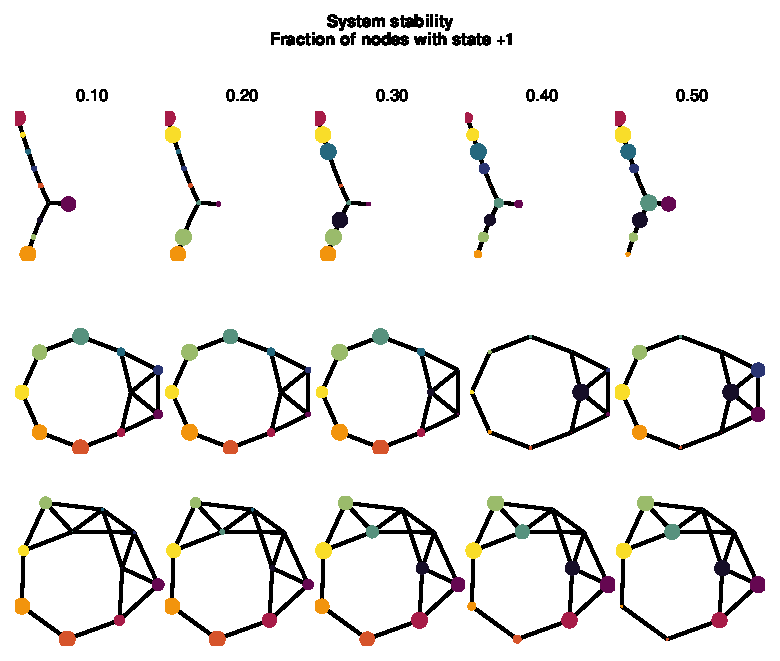
\includegraphics[width=.9\linewidth]{./figures/imi_other_graphs.pdf}
\caption{\label{fig:other_systems}Adjusted mutual information for a random tree (top), and Leder-Coxeter Fruchte graphs (middle, bottom). Each node is goverened by kinetic Ising spin dyanmics. Far away from the tipping point (fraction nodes +1 = 0.5) most information flows are concentrated on non-hub nodes. As the system approaches the tipping point (fraction = 0.5), the information flows move inwards, generating higher adjusted integrated mutual information for nodes with higher degree.}
\end{figure*}

\section{Flip probability per degree}
\label{sec:deg_flip}
In \cref{fig:maj_flip} the tendency for a node
to flip from the majority  to the minority state is computed
as  function of  fraction of  nodes possessing  the majority
states +1  in the system,  denoted as \(N\). Two  things are
observed.   First,  nodes   with  lower   degree  are   more
susceptible to  noise than nodes  with higher degree.  For a
given system stability, nodes with lower degree tend to have
a higher tendency to flip. This is true for all distances of
the system to the tipping point. In contrast, the higher the
degree of  the node, the  closer the system  has to be  to a
tipping point for the node to  change its state. This can be
explained by  the fact that  lower degree nodes,  have fewer
constraints compared to nodes  with higher degree nodes. For
Ising spin kinetics, the nodes with higher degree tend to be
more ``frozen'' in  their node dynamics than  nodes with lower
degree. Second, in order for a node to flip with probability
with similar  mass, i.e.  (\(E[p(s_i) | N]  = 0.2\))  a node
with higher degree  needs to be closer to  the tipping point
than  nodes  with  lower  degree.  In  fact,  the  order  of
susceptibility   is   correlated   with  the   degree;   the
susceptibility  decreases with  increasing degree  and fixed
fraction of nodes in state 1.

\begin{figure}[htbp]
\centering
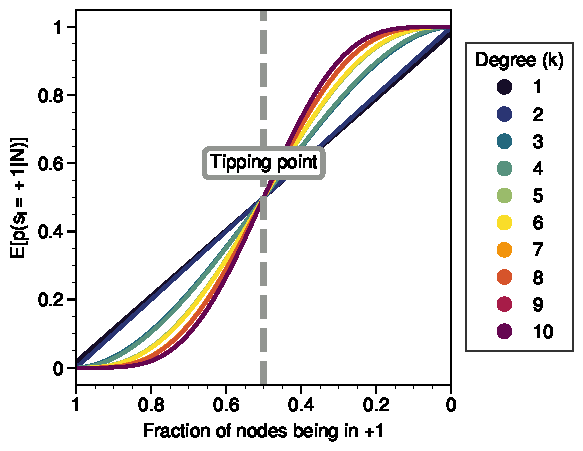
\includegraphics[width=.9\linewidth]{./figures/fig_majority_flip.pdf}
\caption{\label{fig:maj_flip}Susceptibility of a node with degree \(k\) switching from the minority state 0 to the majority state 1 as a function of the neighborhood entropy for \(\beta = 0.5\). The neighborhood entropy encodes how stable the environment of a spin is. As the system approaches the tipping point, the propensity of a node to flip from to the minority state increases faster for low degree nodes than for high degree nodes. Higher degree nodes require more change in their local environment to flip to the majority state. See for details \ref{sec:org009e10c}.}
\end{figure}

\begin{figure*}
\centering
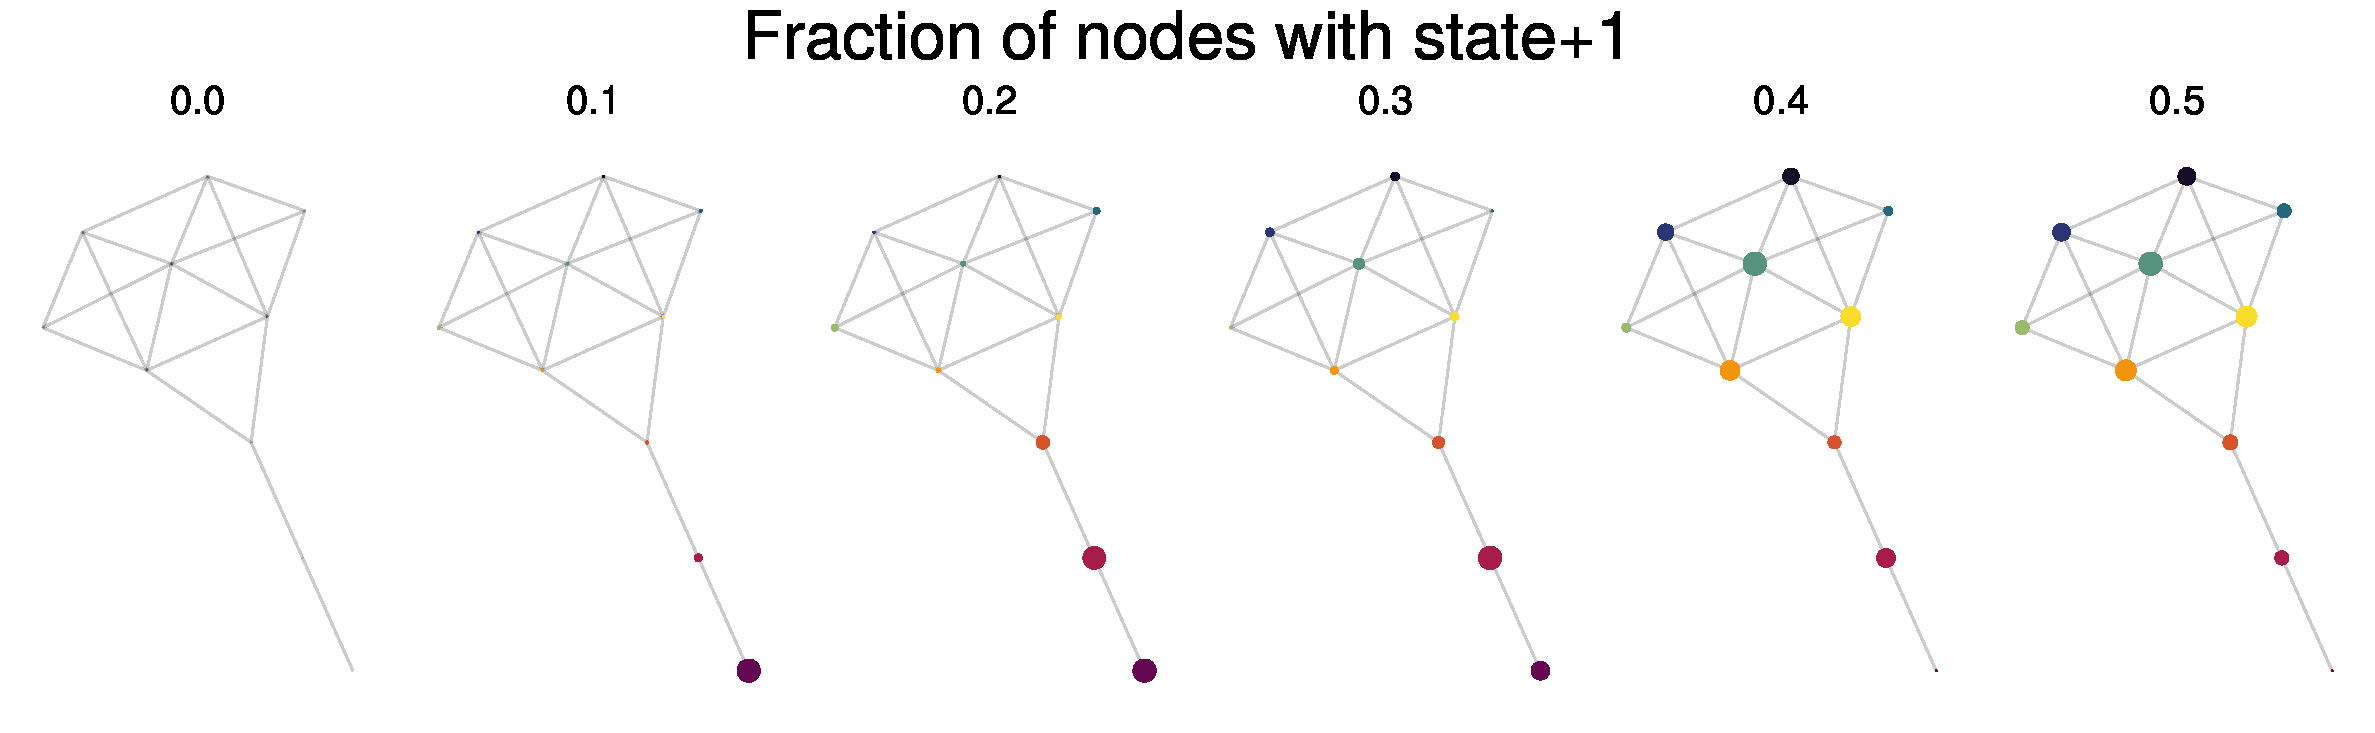
\includegraphics[width=.9\linewidth]{./figures/expectation_kite.pdf}
\caption{\label{fig:expectation_kite}Shortest path analysis of the system ending up in the tipping point from the state where all nodes have state +0. The node size is proportional to the expectation value of a node having state +1  (\(E[s_i = 1]_{S^t, M(S^5)}\) as a function of the fraction of nodes having state +1. The expectation values are computed based on 30240 trajectories, an example trajectory can be seen in \cref{fig:max_trajectory}.}
\end{figure*}
\end{document}
